\documentclass{article}

\usepackage{amsmath,amssymb}
\usepackage{tikz}
\usepackage{pgfplots}
\usepackage{xcolor}
\usepackage[left=2.1cm,right=3.1cm,bottom=3cm,footskip=0.75cm,headsep=0.5cm]{geometry}
\usepackage{enumerate}
\usepackage{enumitem}
\usepackage{marvosym}
\usepackage{tabularx}
\usepackage{parskip}

\usepackage{listings}
\definecolor{lightlightgray}{rgb}{0.95,0.95,0.95}
\definecolor{lila}{rgb}{0.8,0,0.8}
\definecolor{mygray}{rgb}{0.5,0.5,0.5}
\definecolor{mygreen}{rgb}{0,0.8,0.26}
%\lstdefinestyle{java} {language=java}
\lstset{language=R,
	basicstyle=\ttfamily,
	keywordstyle=\color{lila},
	commentstyle=\color{lightgray},
	stringstyle=\color{mygreen}\ttfamily,
	backgroundcolor=\color{white},
	showstringspaces=false,
	numbers=left,
	numbersep=10pt,
	numberstyle=\color{mygray}\ttfamily,
	identifierstyle=\color{blue},
	xleftmargin=.1\textwidth, 
	%xrightmargin=.1\textwidth,
	escapechar=§,
	%literate={\t}{{\ }}1
	breaklines=true,
	postbreak=\mbox{\space}
}

\usepackage[utf8]{inputenc}

\renewcommand*{\arraystretch}{1.4}

\newcolumntype{L}[1]{>{\raggedright\arraybackslash}p{#1}}
\newcolumntype{R}[1]{>{\raggedleft\arraybackslash}p{#1}}
\newcolumntype{C}[1]{>{\centering\let\newline\\\arraybackslash\hspace{0pt}}m{#1}}

\newcommand{\E}{\mathbb{E}}
\DeclareMathOperator{\rk}{rk}
\DeclareMathOperator{\Var}{Var}
\DeclareMathOperator{\Cov}{Cov}

\title{\textbf{Applied Multivariate, Übung 1}}
\author{\textsc{Henry Haustein}}
\date{}

\begin{document}
	\maketitle
	
	\section*{Task 1}
	\begin{lstlisting}
A = matrix(c(1,3,5,3,2,0,5,0,4), 3, 3, byrow = TRUE)
eigen(A)$values
eigen(A)$vectors
gamma = eigen(A)$vectors
lambda = diag(eigen(A)$values)
round(gamma %*% lambda %*% t(gamma))
	\end{lstlisting}
	Die Eigenwerte sind $\lambda_1 = 8.277780$, $\lambda_2 = 2.496552$ und $\lambda_3 = -3.774332$. Die Eigenvektoren sind
	\begin{align}
		v_1 = \begin{pmatrix}
			-0.6208271 \\ -0.2966783 \\ -0.7256416
		\end{pmatrix} \quad v_2 = \begin{pmatrix}
			-0.1435001 \\ -0.8669793 \\ 0.4772365
		\end{pmatrix} \quad v_3 = \begin{pmatrix}
			0.7707019 \\ -0.4004110 \\ -0.4956708
		\end{pmatrix} \notag
	\end{align}
	Damit
	\begin{align}
		\Gamma = \begin{pmatrix}
			-0.6208271 & -0.1435001 & 0.7707019 \\ 
			-0.2966783 & -0.8669793 & -0.4004110 \\ 
			-0.7256416 & 0.4772365 & -0.4956708
		\end{pmatrix} \quad \Lambda = \begin{pmatrix}
			8.277780 & 0 & 0 \\
			0 & 2.496552 & 0 \\
			0 & 0 & -3.774332
		\end{pmatrix} \notag
	\end{align}

	\section*{Task 2}
	\begin{lstlisting}
B = cbind(rnorm(100, mean = 1, sd = 2), 
	rnorm(100), 
	rt(100, df = 4), 
	runif(100, min = 0, max = 4))
pdf("problem1.2.pdf")
boxplot(B)
dev.off()
	\end{lstlisting}
	\begin{center}
		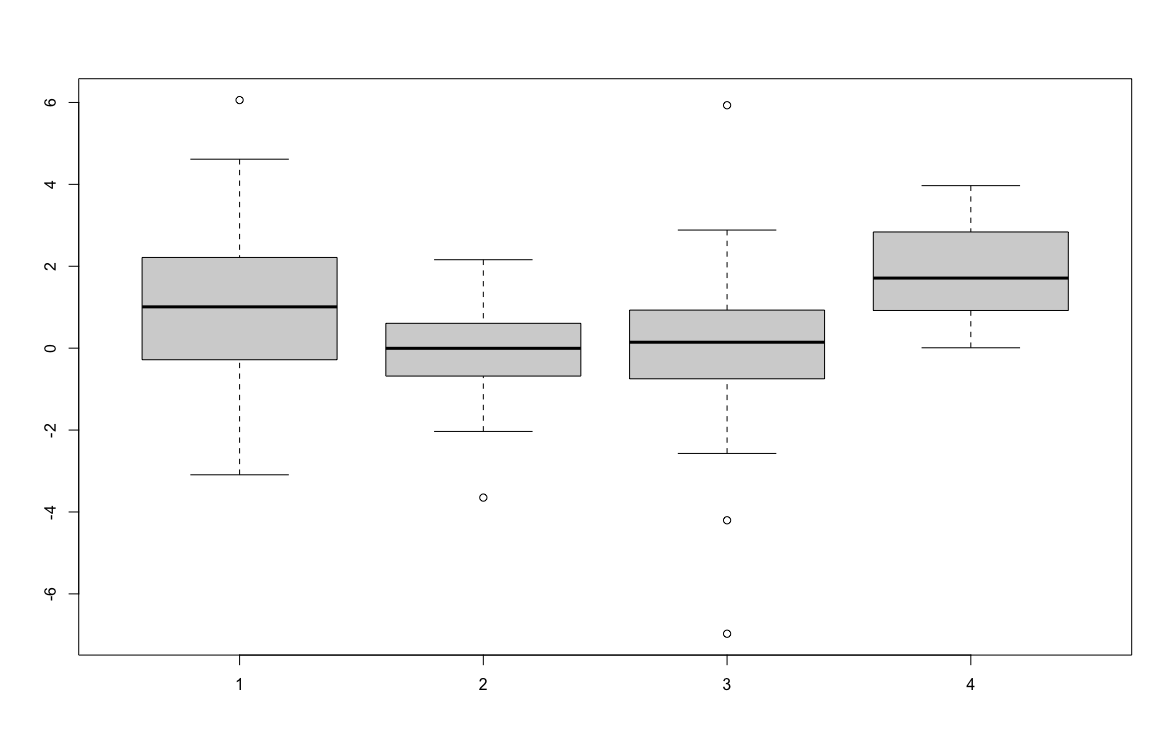
\includegraphics[scale=0.3]{1_2_boxplot}
	\end{center}
	
	\section*{Task 3}
	\begin{lstlisting}
library(ggplot2)
pdf("problem1.3.pdf")
ggplot(iris, aes(x = Sepal.Length, y = Sepal.Width, color = Species)) + geom_point()
dev.off()
cov(iris[,1:4])
	\end{lstlisting}
	\begin{center}
		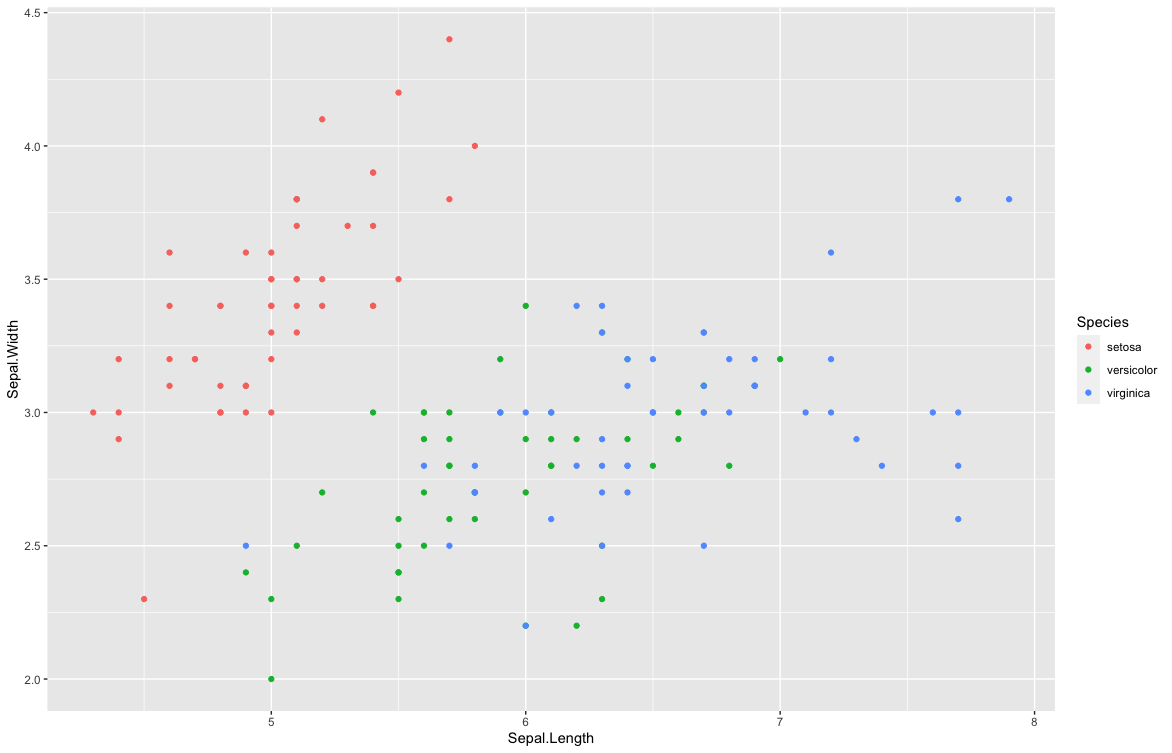
\includegraphics[scale=0.3]{1_3_scatterplot}
	\end{center}
	Und die Kovarianzmatrix ist
	\begin{align}
		\Cov = \begin{pmatrix}
			0.6856935 & -0.0424340 & 1.2743154 & 0.5162707 \\
			-0.0424340 & 0.1899794 & -0.3296564 & -0.1216394 \\
			1.2743154 & -0.3296564 & 3.1162779 & 1.2956094 \\
			0.5162707 & -0.1216394 & 1.2956094 & 0.5810063
		\end{pmatrix} \notag
	\end{align}
	
	\section*{Task 4}
	\begin{lstlisting}
C = matrix(c(1,3,5,3,2,0,7,1,4,1,1,1), nrow = 4, ncol = 3, byrow = TRUE)
lambda = diag(svd(C)$d)
gamma = svd(C)$u
delta = svd(C)$v
round(gamma %*% lambda %*% t(delta))
	\end{lstlisting}
	Liefert
	\begin{align}
		\Gamma &= \begin{pmatrix}
			-0.4784969 & 0.85678269 & 0.08203851 \\
			-0.2919929 & -0.29035642 & 0.88707192 \\
			-0.8106216 & -0.41824208 & -0.40918045 \\
			-0.1693322 & 0.08179326 & 0.19734351
		\end{pmatrix} \quad \Lambda = \begin{pmatrix}
			9.721112 & 0 & 0 \\
			0 & 4.261988 & 0 \\
			0 & 0 & 2.082172
		\end{pmatrix} \notag \\
		 \Delta &= \begin{pmatrix}
			-0.7404667 & -0.6710925 & 0.03666106 \\
			-0.3085481 & 0.3878909 & 0.86852674 \\
			-0.5970822 & 0.6318034 & -0.49428460
		\end{pmatrix} \notag
	\end{align}

\end{document}